\documentclass[aps,onecolumn,twoside,secnumarabic,balancelastpage,amsmath,amssymb,nofootinbib,hyperref=pdftex]{revtex4}


\usepackage{color}         % produces boxes or entire pages with colored backgrounds
\usepackage{graphics}      % standard graphics specifications
\usepackage[pdftex]{graphicx}      % alternative graphics specifications
\usepackage{longtable}     % helps with long table options
\usepackage[english]{babel}
\setlength{\parskip}{1em}
\usepackage{amsmath}
\usepackage{epsf}          % old package handles encapsulated post script issues
\usepackage{bm}            % special 'bold-math' package
\usepackage{verbatim}			% for comment environment
\usepackage[colorlinks=true]{hyperref}  % this package should be added after all others % use as follows: \url{http://web.mit.edu/8.13}                                    
                                  

\begin{document}
\title{}
\author         {Noah Steinberg}
\email          {nastein@umich.edu}
\date{\today}
\affiliation{University of Michigan - Physics}

\maketitle

\section{Suppressing BNV Decays Through Cancellations, An Example}
Consider $p \rightarrow e^{+}\pi^{0}$. The decay rate can be written as a phase-space/kinematic factor multiplied by a combination of powers of Wilson coefficients and the inverse cutoff. Schematically:

\begin{equation}
	\Gamma (p \rightarrow e^{+}\pi^{0}) = K(m_{p}, m_{\pi^0})\frac{C_{eff(p \rightarrow e^{+}\pi^{0})}^2}{\Lambda^4}
\end{equation}


Where K is simply a function of the proton and pion mass, and $C_{eff(p \rightarrow e^{+}\pi^{0})}^2$ contains all the dependence on the heavy degrees of freedom we have integrated out. Given in terms of the Wilson coefficients of the dimension 6 SMEFT operators, for $p \rightarrow e^{+}\pi^{0}$ we have for $C^{2}_{eff(p \rightarrow e^{+}\pi^{0})}$:

\begin{align}
C_{eff(p \rightarrow e^{+}\pi^{0})}^2 & = |C^{1111}_{1}(m_{Z})A_{LR}<\pi^{0}|(ud)_{R}u_{L}|p> - (V_{CKM})_{j1}C^{1j11}_{3}(m_{z})A_{LL}<\pi^{0}|(ud)_{L}u_{L}|p>|^2\\
& + |(V_{CKM})_{j1}[C^{1j11}_{2}(m_{z}) + C^{j111}_{2}(m_{z})]A_{LR}<\pi^{0}|(ud)_{R}u_{L}|p> + C^{1111}_{4}(m_{Z})A_{LL}<\pi^{0}|(ud)_{L}u_{L}|p>|^2
\end{align}

The hadronic matrix elements for the appropriate transitions are evaluated on the lattice at 2 GeV, and typically have uncertainties of $\approx 10$ percent. $A_{LL}$, $A_{LR}$ are renormalization factors for left handed and mixed chirality operators respectively. These renormalization factors allow us to write the Wilson coefficients evaluated at $M_{Z}$, and their value at two loop order is $\approx 1.25$. Super Kamiokande places the lower bound on this proton decay channel at $1.7\times 10^{34}$ years. Naively, order one Wilson coefficients require that $\Lambda$, the scale of BNV physics, be near the GUT scale, $10^{16}$ GeV. At the same time the scale of right handed neutrinos prefers to be at a lower scale of $10^{12} - 10^{14}$ GeV. One might like, instead of two scales appearing in the UV, that there is one scale where $\Lambda_{BNV} = \Lambda_{RHN}$. If we would like the BNV scale near the scale of right handed neutrinos, one requires either unnatural values of the SMEFT Wilson coefficients, or a conspicuous cancellation. 

If we accept that a significant cancellation may occur in the SMEFT Wilson coefficients, the scale of BNV physics can be lowered. Requiring that $\Lambda_{BNV} = 10^{14}$ GeV, $C^{2}_{eff(p \rightarrow e^{+}\pi^{0})}$ must be $\approx 10^{-8}$. If we allow all Wilson coefficients to be of the same order, $\mathcal{O}(10^{-1}) - \mathcal{O}(10^{0})$, then they must differ by small but non vanishing amounts. 

Though highly constrained, $p \rightarrow e^{+}\pi^{0}$ is one of many decay channels searched for. An important fact to remember is that the same Wilson coefficients can contribute to multiple channels. Take for example, $p\rightarrow \pi^{+}\bar{\nu_{i}}$. One finds:

\begin{equation}
C^{2}_{eff(p \rightarrow \pi^{+}\bar{\nu_{i}})} = |-(V_{CKM})_{j1}C^{11ji}_{1}A_{LR}<\pi^{+}|(ud)_{R}d_{L}|p> + (V_{CKM})_{j1}(V_{CKM})_{k1}C^{j1ki}_{3}A_{LL}<\pi^{+}|(ud)_{L}d_{L}|p>|^{2}
\end{equation}


$\Gamma(p\rightarrow \pi^{+}\bar{\nu})$ depends similarly on $C_{1}$ and $C_{3}$ as $\Gamma (p \rightarrow e^{+}\pi^{0})$, with a similar phase space factor, but with different hadronic matrix elements. Requiring $C_{1}$ and $C_{3}$ to have significant cancellation consistent with bounds on $p\rightarrow \pi^{0}e^{+}$, we would like to know if this leads to a similar cancellation for $p\rightarrow\pi^{+}\bar{\nu}$. The degree to which this occurs depends on the the values we use for the hadronic matrix elements. Below we list their values and uncertanties:

\begin{table}[htp]
\caption{Hadronic Matrix Elements for pionic decay channels}
\begin{center}
\begin{tabular}{| |c|c|c|c| |}
\hline
Matrix Element ($\text{GeV}^{3}$) & Central Value\\
\hline\hline
$<\pi^{+}|(ud)_{R}d_{L}|p>$ & -0.186(6)(18)\\
\hline
$<\pi^{+}|(ud)_{L}d_{L}|p>$ & 0.189(6)(22)\\
\hline
$<\pi^{0}|(ud)_{R}u_{L}|p>$ & -0.131(4)(13)\\
\hline
$<\pi^{0}|(ud)_{L}u_{L}|p>$ & 0.134(5)(16) \\
\hline
\end{tabular}
\end{center}
\label{table:hadrons}
\end{table}

 Using the values in table \ref{table:hadrons}, we find $C_{1}$ and $C_{3}$ which satisfy the $p \rightarrow e^{+}\pi^{0}$ bound, and then we check which of these values, if any, will also satisfy the $p\rightarrow \pi^{+}\bar{\nu_{i}}$ constraint. For the moment we ignore CKM mixing.


\begin{figure}[htbp]
\begin{center}
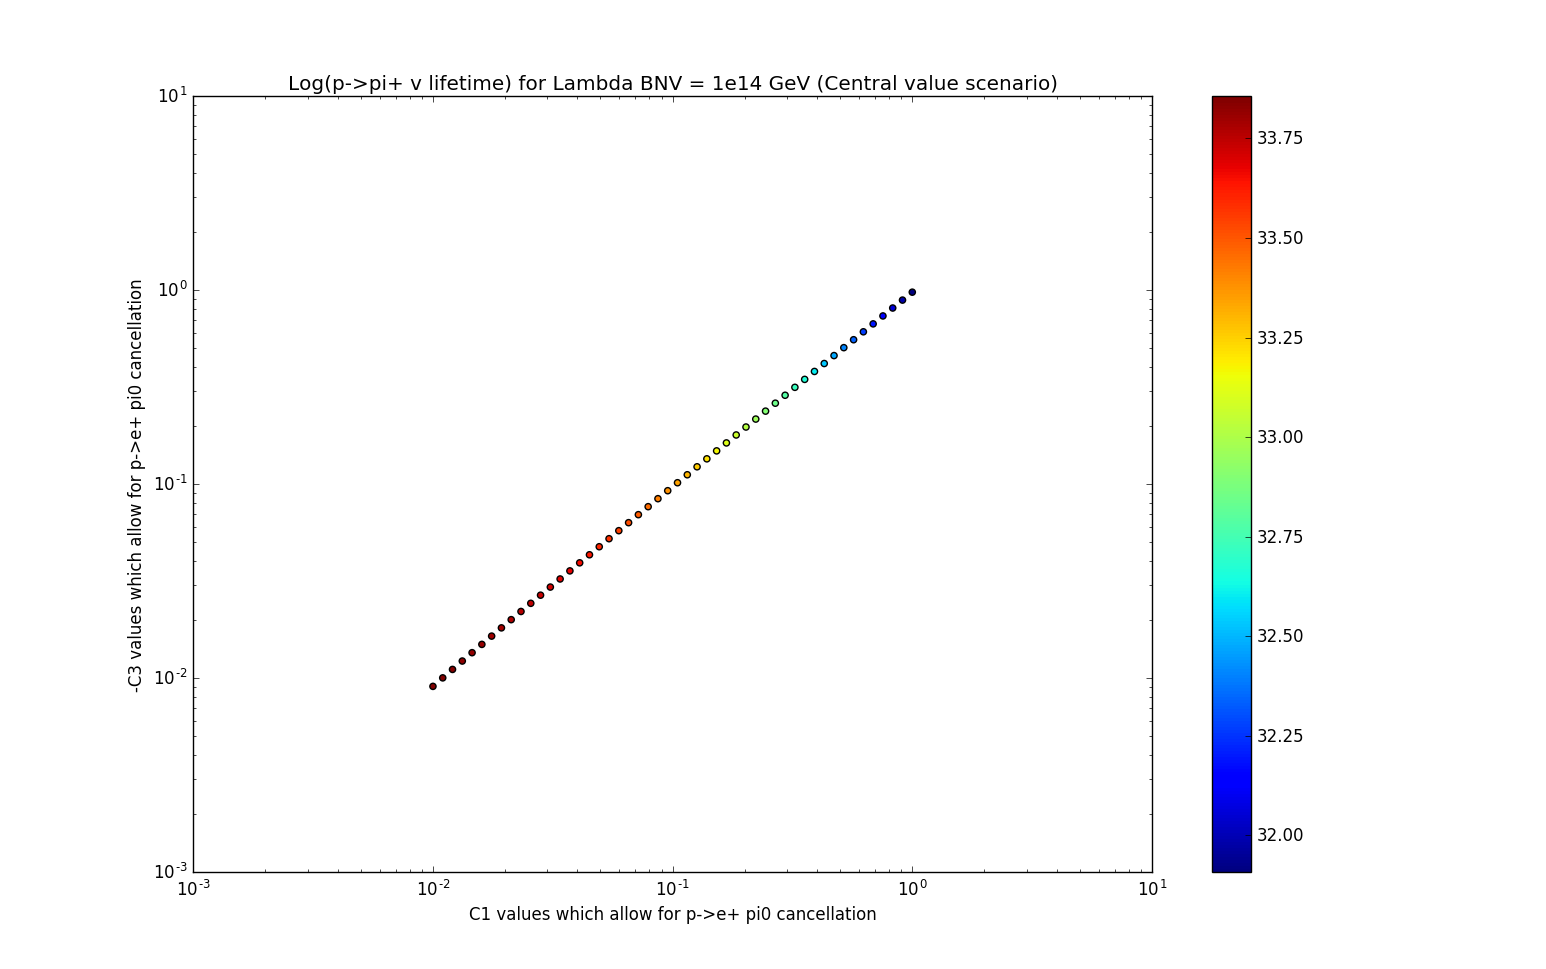
\includegraphics[width=18cm]{central_value.png}
\caption{Values of $C_1$ and $-C_3$ which satisfy the Super Kamiokande $p \rightarrow e^{+}\pi^{0}$ constraint. The color bar on the right shows the predicted value of $\text{Log}_{10}(\tau_{p\rightarrow \pi^{+}\bar{\nu_{i}}}/\text{years})$ as a function of $C_1$ and $-C_3$. The lower lifetime given by Super Kamiokande is $3.9\times10^{32}$ years.}
\label{figure:1}
\end{center}
\end{figure}

Figure \ref{figure:1} shows the result of this calculation. Both proton decay constraints can be satisfied with $\mathcal{O}(10^{-1})$ values for the Wilson coefficients. The maximum allowed value of the Wilson coefficients depends on the value we use for the hadronic matrix elements. We have checked that within their given uncertainties, results for the upper bound on the size of $|C_1|$ and $|C_3|$ do not change much. 

















\end{document}